\documentclass[12pt]{article}

\usepackage{graphicx}
\usepackage{paralist}
\usepackage{listings}
\usepackage{booktabs}
\usepackage{hyperref}
\usepackage{amsfonts}
\usepackage{amsmath}
\usepackage{amssymb}
\usepackage{pdfpages}
\usepackage{graphicx}

\graphicspath{ {./images/} }
\oddsidemargin 0mm
\evensidemargin 0mm
\textwidth 160mm
\textheight 200mm

\pagestyle {plain}
\pagenumbering{arabic}
\newcounter{stepnum}
\newcommand\tab[1][1cm]{\hspace*{#1}}

\title{Assignment 4 Design Specification}
\author{SFWRENG 2AA4}
\date{\today}

\begin {document}
\maketitle
%Source for most of the introductory info is Wikipedia, a lot of the wording should be similar between the two.
% https://en.wikipedia.org/wiki/2048_(video_game)

% https://gitlab.cas.mcmaster.ca/smiths/se2aa4_cs2me3/-/blob/master/Assignments/PreviousYears/2020/A4-Dots/A4Soln/Design%20Specification/spec.pdf

%https://www.washingtonpost.com/news/arts-and-entertainment/wp/2014/04/23/everything-you-ever-wanted-to-know-about-2048-the-internets-latest-impossible-hit-game/

% https://play2048.co/

This Module Interface Specification (MIS) document will contain various modules, types and methods that are needed for the implementation of the game \emph{2048}. Throughout this specification the word cell will be used to refer to space occupied by each tile in the grid. At the start of the game the user has a 4 x 4 grid with numbered tiles that will slide across the board as the user moves them with arrow keys. After every new click of the arrow, a new tile will appear in a random empty square in the board. This tile will have the value of 2 or 4. As the arrow keys move, the tiles will slide as far as is possible in the direction of the arrow key unless they are impeded by the boundary of the grid or by another tile. If two tiles of the same value collide during the sliding process, a new tile will form that is the sum of the previous tiles. Tiles can only merge in groups of two. The game is considered \emph{finished} or \emph{won} when the board is full and the player has no more moves or when a tile with the value \emph{2048} is on the board, respectively. 

\begin{center}
	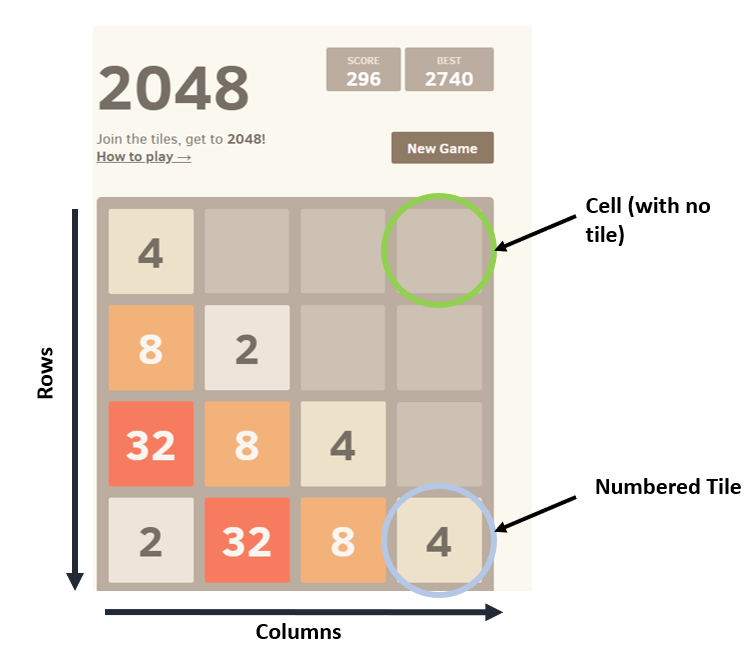
\includegraphics[scale = 0.70]{IntroToTerm.png}
\end{center}
\newpage

\section* {Overview of the design}
% This section nis also heavily influenced by the given specification: https://gitlab.cas.mcmaster.ca/smiths/se2aa4_cs2me3/-/blob/master/Assignments/PreviousYears/2020/A4-Dots/A4Soln/Design%20Specification/spec.pdf

This design applies the Model-View-Controller (MVC) design pattern and Singleton design pattern. The MVC components are comprised of $BoardT$ which is the model module and $UserInterface$ which is the view module. The Singleton design pattern makes an appearance when getting the abstract object for the $UserInterface$ module. \newline

The implementation of the MVC design pattern is as follows:
\begin{itemize}
    \item $BoardT$ stores the state of the game board and all methods to make changes to the board throughout the game. 
    \item $UserInterface$ displays the state of the game board using text-based graphics that are output to the screen. 
\end{itemize}

Below is the UML diagram for visualizing this software architecture. The Game Controller is just for show. An actual game controller was not made as part of this MIS. 

% UML created at:
% https://online.visual-paradigm.com/drive/#diagramlist:proj=0&new=ClassDiagram
\begin{center}
	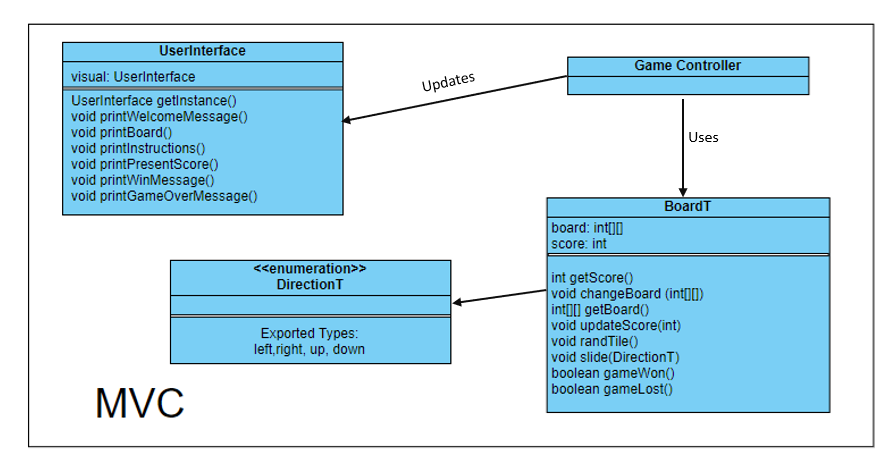
\includegraphics[scale = 0.5]{mvcUML.jpeg}
\end{center}


\section* {Likely changes my design considers}
\begin{itemize}
    \item The design also considers the changing of displayed text as the user can go from win to loss to seeing the score and the board.
\end{itemize}
\newpage
% Made use of:
% https://gitlab.cas.mcmaster.ca/smiths/se2aa4_cs2me3/-/blob/master/Assignments/A3/A3P1_Spec.tex
\section* {DirectionT Module}

\subsection*{Module}
DirectionT

\subsection* {Uses}

None

\subsection* {Syntax}

\subsubsection* {Exported Constants}

None

\subsubsection* {Exported Types}

DirectionT = \{\\
    right, \textit{\#Sliding to the right}\\
    left, \textit{\#Sliding to the left}\\
    up, \textit{\#Sliding upwards}\\
    down, \textit{\#Sliding downwards}\\
\} $//$ Use enums to implement in Java

\subsubsection* {Exported Access Programs}

None

\subsection* {Semantics}

\subsubsection* {State Variables}

None

\subsubsection* {State Invariant}

None

\subsubsection* {Assumptions}

None

\newpage



%Here begins BoardT

\section* {BoardT ADT Module}

\subsection* {Template Module}

BoardT

\subsection* {Uses}

Not sure yet

\subsection* {Syntax}

\subsubsection* {Exported Types}

None

\subsubsection* {Exported Constants}

None

\subsubsection* {Exported Access Programs}

\begin{tabular}{| l | l | l | p{6cm} |}
\hline
\textbf{Routine name} & \textbf{In} & \textbf{Out} & \textbf{Exceptions}\\
\hline
new BoardT & ~ & BoardT &  \\
\hline
getScore & ~ & $\mathbb{N}$ & \\
\hline
changeBoard & seq [4, 4] of $\mathbb{N}$& ~ &\\
\hline
getBoard & ~ & seq [4, 4] of $\mathbb{N}$ & \\
\hline
updateScore & $\mathbb{N}$ & ~ & \\
\hline
randTile & ~ & ~ & \\
\hline
slide & DirectionT & ~ & \\
\hline
gameWon & ~ & $\mathbb{B}$ & \\
\hline
gameLost & ~ & $\mathbb{B}$ & \\
\hline
\end{tabular}

\subsection* {Semantics}

\subsubsection* {State Variables}

$board$: seq [4, 4] of $\mathbb{N}$\newline
$score$: $\mathbb{N}$

\subsubsection* {State Invariant}

None

\subsubsection* {Assumptions}

\begin{itemize}
\item It is assumed that throughout the module the tile order (general order of tiles in rows and columns) remains the same. This interpretation will not change even if tiles are merged. It is assumed that the constructor is called before any other access routine and is only called once. It is also assumed that changeBoard() will only be used for testing purposes. 
\end{itemize}
\subsubsection* {Access Routine Semantics}

\noindent new BoardT():
\begin{itemize}
  \item transition: board, score $:=$ $\langle \langle 0,0,0,0 \rangle,\langle 0,0,0,0 \rangle, \langle 0,0,0,0\rangle, \langle 0,0,0,0 \rangle \rangle$,  0\newline
  \item output: $out$ $:=$ \textit{self}
  \item exception: None
\end{itemize}

\noindent getScore():
\begin{itemize}
\item output: $out$ $:=$ $score$ 
\item exception: None
\end{itemize}

\noindent changeBoard($matrix$):
\begin{itemize}
\item transition: $board$ $:=$ $b$ $\#$ This will only be used for testing purposes.
\item exception: None
\end{itemize}

\noindent getBoard():
\begin{itemize}
\item transition: $out$ $:=$ $board$.
\item exception: None
\end{itemize}

\noindent updateScore($tile$):
\begin{itemize}
\item transition: $score$ $:=$ $score$ + $tile$
\item exception: None
\end{itemize}

\noindent randTile():
\begin{itemize}
\item transition: ($\lnot (value = random (2,4)) = 3) \land ( i = random(0,3) \land j = random(0,3)) \land board[i][j] = 0)   \Rightarrow board[i][j] := value$ \newline \textit{$\#$ Check if the value of the random tile is not either 2 or 4 and that the random cell doesn't already have a tile. If these two conditions are met, place the random tile in the random cell.}\\
\item exception: None\newline
\end{itemize}

\noindent slide($direction$):
\begin{itemize}
\item transition: ($direction = left \Rightarrow board := (slideLeft(), mergeLeft(), slideLeft() ) )$ $|$
$(direction = right \Rightarrow board := (slideRight(), mergeRight(), slideRight()))$ $|$
$(direction = up \Rightarrow board := (slideUp(), mergeUp(), slideUp()))$ $|$
$(direction = down \Rightarrow board := (slideDown(), mergeDown(), slideDown()))$
\item exception: None
\end{itemize}

\noindent gameWon():
\begin{itemize}
\item output: $out := (\exists i, j :  \mathbb{N} |$ $i, j \in [0...3] \land (board[i][j] \ge 2048))$
\item exception: None\newline
\end{itemize}

\noindent gameLost():
\begin{itemize}
\item output: $out := \lnot (\exists i, j :  \mathbb{N} |$ $i, j \in [0...3] : areStillMoves(i, j))$
\item exception: None\newline
\end{itemize}

\subsection*{Local Functions}

\noindent $\mbox{fullBoard}: \rightarrow \mathbb{B}$\\
\noindent
$\mbox{fullBoard} \equiv \langle (\forall i, j :  \mathbb{N} | i, j \in board : \lnot (board[i][j] ==0) )\rangle$
\textit{$\#$Return whether or not the board is full of tiles.}
~\\

\noindent $\mbox{canMerge}: \mathbb{N} \times \mathbb{N} \rightarrow \mathbb{B}$\\
\noindent $\mbox{canMerge}(i, j) \equiv \langle i, j :  \mathbb{N} | i, j \in board : (board[i][j] == board[i][j+1] | board[i][j] == board[i][j-1] | board[i][j] == board[i+1][j] | board[i][j] == board[i-1][j])\rangle$ \newline

\noindent $\mbox{slideLeft}:$ \textit{$\#$ Has no input or output, runs a state change}\\
\noindent $\mbox{slideLeft} \equiv board := (\forall i, j :  \mathbb{N} |$ $i, j \in [0...3]) \Rightarrow$  Check that the current cell does not have a tile (value of 0) and travelling to the left of the board (column index decreases), check whether there are empty spaces for the current tile to slide to the left, the slide the tiles. \newline

\noindent $\mbox{slideRight}:$ \textit{$\#$ Has no input or output, runs a state change}\\
\noindent $\mbox{slideRight} \equiv board := (\forall i, j :  \mathbb{N} |$ $i \in [0...3] \land j \in [3...0] ) \Rightarrow$  Check that the current cell does not have a tile (value of 0) and travelling to the right of the board (column index increasing), check whether there are empty spaces for the current tile to slide to the right, then slide the tiles. \newline

\noindent $\mbox{slideUp}:$ \textit{$\#$ Has no input or output, runs a state change}\\
\noindent $\mbox{slideUp} \equiv board := (\forall i, j :  \mathbb{N} |$ $i, j \in [0...3]) \Rightarrow$  Check that the current cell does not have a tile (value of 0) and travelling upwards on the board (row index decreases), check whether there are empty spaces for the current tile to slide upwards, then slide the tiles. \newline

\noindent $\mbox{slideDown}:$ \textit{$\#$ Has no input or output, runs a state change}\\
\noindent $\mbox{slideDown} \equiv board := (\forall i, j :  \mathbb{N} |$ $i \in [0...3] \land j \in [3...0] ) \Rightarrow$  Check that the current cell does not have a tile (value of 0) and travelling downwards on the board (row index increasing), check whether there are empty spaces for the current tile to slide to downwards, then slide the tiles. \newline

\noindent $\mbox{mergeLeft}:$ \textit{$\#$ Has no input or output, runs a state change}\\
\noindent $\mbox{mergeLeft} \equiv ((\forall i, j :  \mathbb{N} |$ $i, j \in [0...3]) \land (board[i][j] = board[i][j+1])) \Rightarrow merge(i, j, i, j+1)$  \newline

\noindent $\mbox{mergeRight}:$ \textit{$\#$ Has no input or output, runs a state change}\\
\noindent $\mbox{mergeRight} \equiv ((\forall i, j :  \mathbb{N} |$ $i \in [0...3] \land j \in[3..0]) \land (board[i][j] = board[i][j-1])) \Rightarrow merge(i, j, i, j-1)$ \newline

\noindent $\mbox{mergeUp}:$ \textit{$\#$ Has no input or output, runs a state change}\\
\noindent $\mbox{mergeUp} \equiv ((\forall i, j :  \mathbb{N} |$ $i, j \in [0...3]) \land (board[i][j] = board[i+1][j])) \Rightarrow merge(i, j, i+1, j)$  \newline

\noindent $\mbox{mergeDown}:$ \textit{$\#$ Has no input or output, runs a state change}\\
\noindent $\mbox{mergeDown} \equiv ((\forall i, j :  \mathbb{N} |$ $i \in [0...3] \land j \in[3..0]) \land (board[i][j] = board[i-1][j])) \Rightarrow merge(i, j, i-1, j)$ \newline

\noindent $\mbox{merge}:\mathbb{N} \times \mathbb{N} \times \mathbb{N} \times \mathbb{N} \rightarrow $\\
\noindent $\mbox{merge}(row, col, row1, col1) \equiv \langle (board[row][col] = board[row][col] + board[row][col]) \land board[row1][col1] = 0 \rangle$\\

\noindent $\mbox{random}:\mathbb{N} \times \mathbb{N} \rightarrow \mathbb{N}$ \\
\noindent $\mbox{random}(num1, num2) \equiv$ outputs a random number between num1 and num2 inclusive. 

\newpage

% A great portion of the following section of the specification can be attributed to the sample specification given to us:
% https://gitlab.cas.mcmaster.ca/smiths/se2aa4_cs2me3/-/blob/master/Assignments/PreviousYears/2020/A4-Dots/A4Soln/Design%20Specification/spec.pdf

\section* {UserInterface Module}

\subsection* {UserInterface Module}

\subsection* {Uses}

None

\subsection* {Syntax}

\subsubsection* {Exported Types}

None

\subsubsection* {Exported Constants}

None

\subsubsection* {Exported Access Programs}

\begin{tabular}{| l | l | l | p{6cm} |}
\hline
\textbf{Routine name} & \textbf{In} & \textbf{Out} & \textbf{Exceptions}\\
\hline
getInstance & ~ & UserInterface &  \\
\hline
printBoard & int[][] & ~ & \\
\hline
printInstructions & ~ & ~ & \\
\hline
printWelcomeMessage & ~ & ~ & \\
\hline
printPresentScore & BoardT & ~ & \\
\hline
printWinMessage & ~ & ~ & \\
\hline
printGameOverMessage & ~ & ~ & \\
\hline
\end{tabular}

\subsection* {Semantics}

\subsection*{Environment Variables}

$window$: A portion of computer screen to display the game and messages

\subsubsection* {State Variables}

$visual$: UserInterface

\subsubsection* {State Invariant}

None

\subsubsection* {Assumptions}

\begin{itemize}
\item The constructor is called for each object instance before any
other access routine is called for that object and it is only called once.
\end{itemize}
\subsubsection* {Access Routine Semantics}

\noindent getInstance():
\begin{itemize}
  \item transition: visual $:=$ (visual = null $\Rightarrow$ new UserInterface())
  \item output out $:=$ \textit{self}
  \item exception: None
\end{itemize}


\noindent printBoard($board$):
\begin{itemize}
\item transition: window $:=$ Draws the game board onto the screen. The board is accessed using the $getBoard$ method from $BoardT$. The board[x][y] is displayed so that x increases from the left of the screen to the right, and y increases from the top to the bottom of the screen. For example, board[0][0] is displayed at the top-left corner and board[3][3] is displayed at bottom-right corner. 
\end{itemize}

\noindent printInstructions():
\begin{itemize}
\item transition: window $:=$ Displays the game instructions to the screen.
\end{itemize}

\noindent printWelcomeMessage():
\begin{itemize}
\item transition: window $:=$ Displays a message that welcomes the user.
\end{itemize}

\noindent printPresentScore($board$):
\begin{itemize}
\item transition: window $:=$ Displays a message showing the user's score using board.getScore().
\end{itemize}

\noindent printWinMessage():
\begin{itemize}
\item transition: window $:=$ Displays a message to congratulate the user when they get the tile 2048.
\end{itemize}

\noindent printGameOverMessage():
\begin{itemize}
\item transition: window $:=$ Displays a message to tell the user the game is over when the 4 x 4 board is full of tiles and no further moves can be made.
\end{itemize}
\newpage

\section* {Critique of Design}
\begin {itemize}
    \item The $UserInterface$ module is specified as an abstract object as we only need a singular instance of the view to be used alongside a controller during the runtime. As such, there will be no possibility for changing state. 
    \item The $BoardT$ module is specified as an ADT because it seems a better choice to create a new instance of BoardT when restarting or after losing a game.
    \item The majority of my methods are essential, they all serve a purpose and are divided so as to serve a single purpose at a time. By combining them, the modules as a whole are cohesive and complete.
    \item The separation of sliding and merging into methods for each direction is not considered essential. The reason I did this is for maintainability and verifiability. By separation of concerns, creating more methods allowed for me to more easily verify if the code was reliable and correct. In part the MVC design pattern also contributes to the maintainability by keeping related methods together in modules. \newline
    Note: If there was something specifically wrong with merging or sliding tiles, it would be easy to find where the error occured. 
    \item In terms of minimality, the specification ensures that different services are not offered by the same access program. I made sure that I did so even at the risk of essentiality at times. This is shown by the fact that every single move on the board, whether it be sliding, merging or updating score, has its own access program. This is especially prominent in the UserInterface module where all the printing methods are separated by content. 
    \item Following off the previous point, I also ensured consistency by naming the methods that worked together similarly, as shown below:
        \begin{itemize} %The double itemization was shown to me by Farzan Yazdanjou
            \item  slideUp(), slideLeft(), slideDown(), slideRight()
            \item  mergeUp(), mergeLeft(), mergeDown(), mergeRight()
            \item  printBoard(), printScore()...
        \end{itemize}
    \item The MIS could have been more general in the sense that the board could have been able to work with different board size. Unfortunately, that implementation would have changed a lot of the methods I had made previously, so I had decided not to include that. However, the methods made for shifting in different directions was made general, in the sense that, had I chosen to allow for varying sizes in the board, they would be able to update easily with that change. In particular, these methods rely on board.length which is subject to change depending on what length was specified by the code.
    %Here I made particular use of the examples in the A4 that was given.
    \item As for information hiding/opacity, though the methods for making the tiles slide are public, the access programs that actually allow for the sliding and merging motions are all private e.g. (slideUp(), mergeLeft(), etc...). This enforces information hiding because the implementation information that is not necessary for the user is not made easily accessible and remains hidden in the background.
    \item This MIS design achieves high cohesion low coupling  through the application of the MVC design pattern. The related functionalities are kept together in the model, and view parts of the design respectively. This enables high cohesion. As for low coupling, the controller would  with both model and view but for the most part the implementations are independent of one another. Therefore, a change to any individual module does not severely damage any of the others.
\end{itemize}

\newpage

\section* {Answers to Questions}
\begin{enumerate}
\item Please see the folder for UMLQ1.jpeg, the photo is too large to be implemented here. Any attempts to resize ruined the quality of the image.
\end{enumerate}

% Source forinformation about the UMLs:
% https://taylorial.com/cs1021/UMLClass.htm#:~:text=A%20class%20implementing%20an%20interface,the%20class%20that%20is%20used. 
% \begin{center}
% \noindent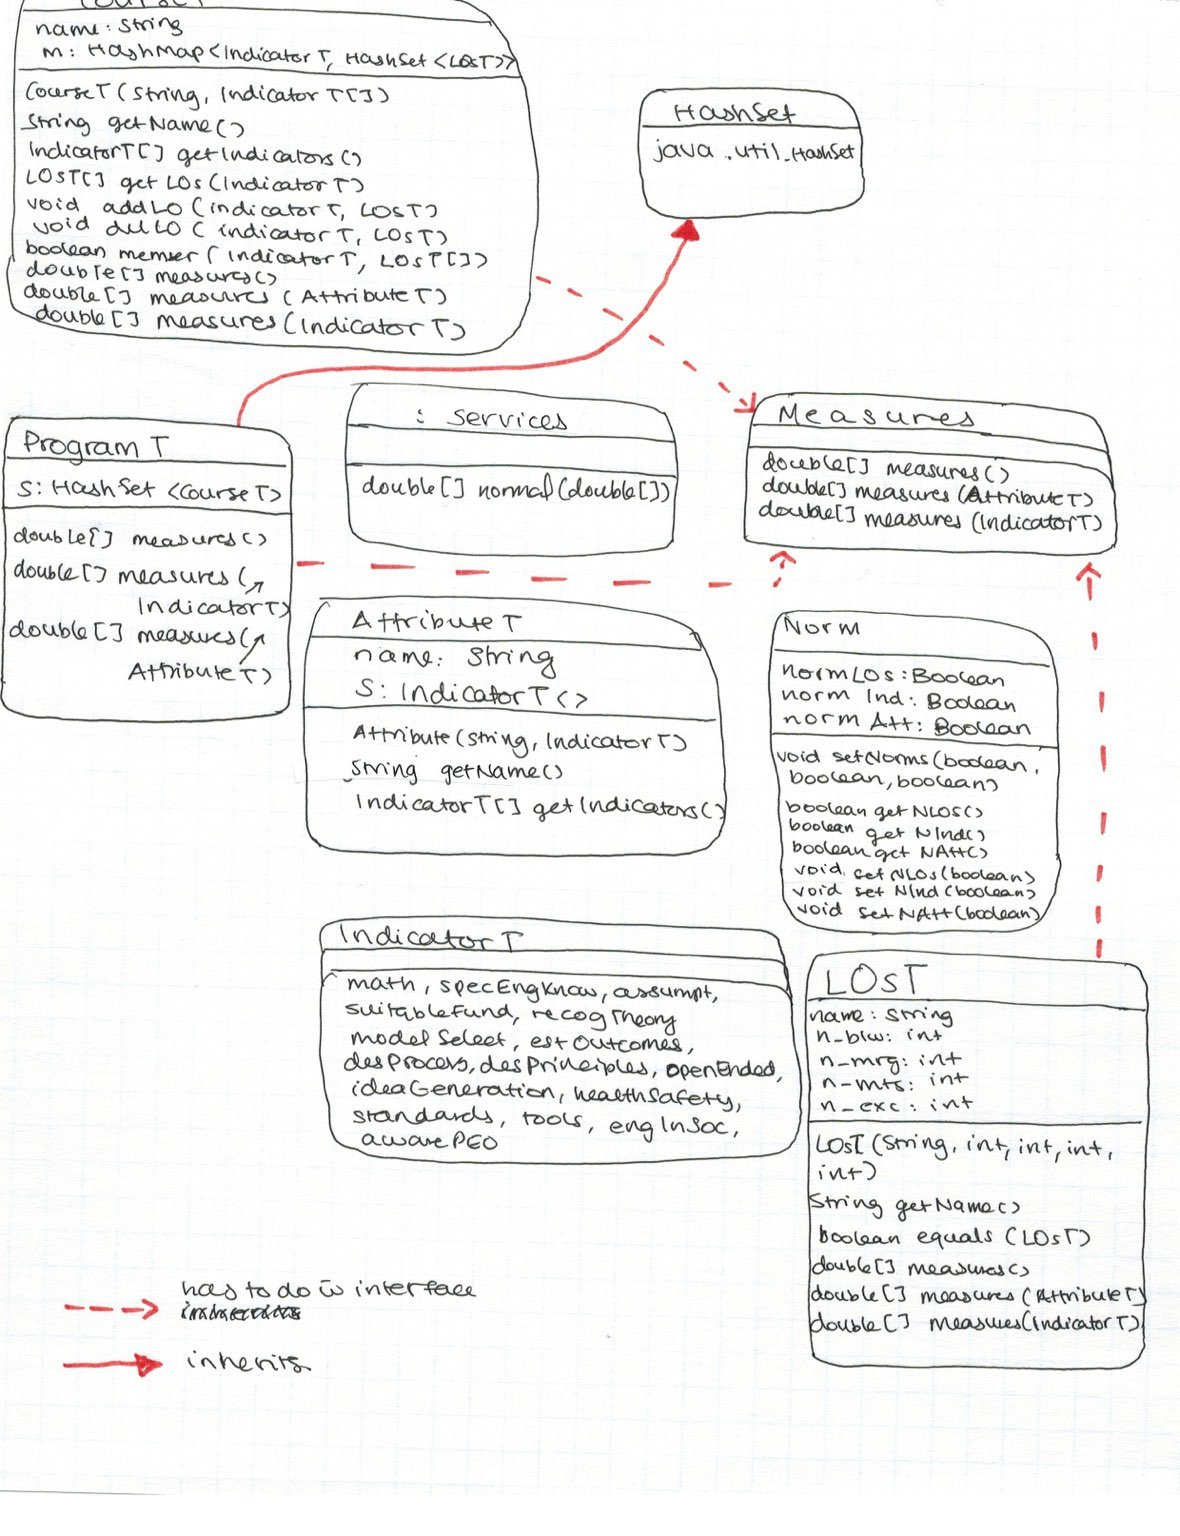
\includegraphics[scale=0.0, angle = 180, origin = c]{UMLQ1.jpeg}
% \end{center} 

\end {document}
